\section{One-Click Checkout Architecture}


\subsection{Customer Recognition}

Rapid customer identification enables one-click checkout. We employ a multi-signal recognition system:

\begin{equation}
identity(request) = \begin{cases}
    c_{token} & \text{if } session\_token \in request \\
    c_{device} & \text{if } device\_fingerprint \in \mathcal{D}_c \\
    c_{email} & \text{if } email\_hash \in \mathcal{E}_c \\
    \bot & \text{otherwise}
\end{cases}
\end{equation}

\begin{algorithm}
\caption{Customer Recognition}
\begin{algorithmic}[1]
\Function{IdentifyCustomer}{$request$}
    \If{$request.sessionToken \neq \bot$}
        \State $c \gets$ \Call{LookupSession}{$request.sessionToken$}
        \If{$c \neq \bot$} \Return $c$ \EndIf
    \EndIf
    \State $fingerprint \gets$ \Call{ComputeFingerprint}{$request$}
    \State $c \gets$ \Call{LookupFingerprint}{$fingerprint$}
    \If{$c \neq \bot \land confidence(c) > \theta$}
        \State \Return $c$
    \EndIf
    \If{$request.email \neq \bot$}
        \State \Return \Call{LookupEmail}{$hash(request.email)$}
    \EndIf
    \State \Return $\bot$
\EndFunction
\end{algorithmic}
\end{algorithm}

\subsection{Token Management}

Payment tokens abstract sensitive credentials:

\begin{definition}[Payment Token]
A payment token $p$ is a tuple $(id, type, last4, exp, scope)$ where:
\begin{itemize}
    \item $id$: unique token identifier
    \item $type \in \{CARD, BANK, WALLET\}$: payment method type
    \item $last4$: last four digits for display
    \item $exp$: expiration timestamp
    \item $scope \subseteq \mathcal{M}$: authorized merchants
\end{itemize}
\end{definition}

Tokens are stored in an isolated vault with the following security invariant:

\begin{theorem}[Token Isolation]
For any token $p$ and merchant $m$, access to the underlying credential requires:
\[
access(p, m) \Rightarrow m \in p.scope \land valid(p) \land authenticated(m)
\]
\end{theorem}

\subsection{One-Click Flow}

The complete one-click checkout executes in three phases:

\begin{enumerate}
    \item \textbf{Recognition} (< 50ms): Customer identified via session or fingerprint
    \item \textbf{Authorization} (< 100ms): Payment authorized with stored token
    \item \textbf{Confirmation} (< 50ms): Order confirmed and receipt generated
\end{enumerate}

\begin{figure}[h]
\centering
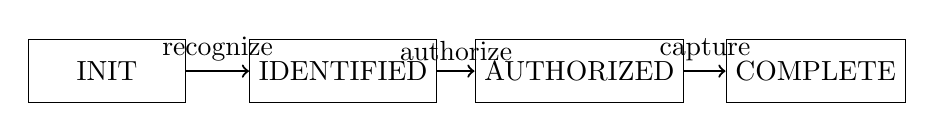
\begin{tikzpicture}[
    node distance=2cm,
    state/.style={rectangle, draw, minimum width=2cm, minimum height=0.8cm},
    arrow/.style={->, thick}
]
    \node[state] (init) {INIT};
    \node[state, right of=init, xshift=1cm] (ident) {IDENTIFIED};
    \node[state, right of=ident, xshift=1cm] (auth) {AUTHORIZED};
    \node[state, right of=auth, xshift=1cm] (complete) {COMPLETE};

    \draw[arrow] (init) -- node[above] {recognize} (ident);
    \draw[arrow] (ident) -- node[above] {authorize} (auth);
    \draw[arrow] (auth) -- node[above] {capture} (complete);
\end{tikzpicture}
\caption{One-click checkout state transitions}
\end{figure}

